\documentclass[conference]{IEEEtran}
\usepackage{cite}
\usepackage{amsmath,amssymb}
\usepackage{graphicx}
\usepackage{booktabs}
\usepackage{xcolor}
\usepackage{tikz}
\usetikzlibrary{arrows.meta,positioning,fit,shapes.misc}
\usepackage{listings}
\usepackage[hidelinks]{hyperref}
\lstset{basicstyle=\ttfamily\scriptsize,breaklines=true,frame=single,columns=fullflexible}
% \pending{...} prints red placeholder text (author names / affiliation). Fill them in, then remove the macro before submission.
\newcommand{\pending}[1]{\textcolor{red}{[#1]}}

\begin{document}

\title{KAVACH: A Model-Agnostic, Intent-Aware Jailbreak Defence Layer for LLMs with Tactic--Harm Decoupling and Hindi--Hinglish Canonicalization}

\author{\IEEEauthorblockN{Vaibhavi Das\IEEEauthorrefmark{1} \pending{co-authors / supervisor}}
\IEEEauthorblockA{\IEEEauthorrefmark{1}\pending{Department, Institution, City, India}\\
vaibhavidasv2005@gmail.com}}

\maketitle

\begin{abstract}
LLM safety mechanisms can be bypassed by \emph{jailbreak} prompts that wrap a harmful request in role-play, hypothetical framing, instruction overrides or obfuscation. Such attacks are especially effective in regional and code-mixed languages such as Hindi and romanized Hinglish. Existing guard models depend on their training data and decide with a binary allow/refuse output, which also refuses many legitimate prompts that merely \emph{look} like attacks. We present \textsc{Kavach}, a plug-in safety layer that wraps any LLM through a Python API or an OpenAI-compatible proxy; its core needs no training data. \textsc{Kavach} (i)~canonicalizes inputs by transliterating Devanagari, mapping Hinglish spelling variants to phonetic keys and decoding obfuscation; (ii)~scores \emph{what} is asked (harm) separately from \emph{how} it is asked (evasion tactic); (iii)~sends uncertain prompts to an LLM judge driven by \emph{Intent Decomposition Prompting}, which removes the framing and rates the bare core request; and (iv)~chooses among six graded actions, from answering under a hardened prompt to redirecting to a safe rewrite or blocking, with an adaptive attack memory and conversation-level risk tracking. On a 4{,}648-prompt held-out test set drawn from seven public sources in seven Indian languages, decoupling cuts false refusals of benign in-the-wild prompts from 11.1\% for a tactic-based detector to 0.2\%, while the model-free stage routes 71.8\% of harmful prompts to the judge. Removing transliteration drops Hindi routing recall from 64.3\% to 0\%. With Gemini~3.5 Flash-Lite as judge on a stratified 186-prompt sample, the IDP judge refuses 81.2\% of harmful prompts and intervenes on 90.6\% with no false refusals. A naive yes/no judge on the same model refuses about the same share overall (80.9\%) but does worse on India-specific harms (73.8\% vs.\ 88.1\%), multi-turn jailbreaks (85.7\% vs.\ 95.2\%) and romanized Hindi (50.0\% vs.\ 75.0\%). Finally, we fine-tune multilingual transformers as the cascade's router. XLM-R raises routing recall from 71.8\% to 95.0\% while sending 58\% fewer benign prompts to the judge, and the learned cascade refuses 74--80\% of harmful prompts end to end, up from 62.4\%.
\end{abstract}

\begin{IEEEkeywords}
LLM safety, jailbreak defence, prompt engineering, guardrails, multilingual NLP, code-mixing, Hinglish
\end{IEEEkeywords}

\section{Introduction}
Large language models (LLMs) are now part of customer support, education, health and government services, where they must answer a wide range of queries safely. Safety alignment remains brittle. Jailbreak prompts exploit \emph{competing objectives}, for example ``stay in character'', and \emph{mismatched generalisation}, for example encodings or low-resource languages the safety training never covered~\cite{wei2023jailbroken}. In-the-wild jailbreak communities produce new templates continuously~\cite{shen2024dan}, and translating a harmful request into a low-resource language raises attack success sharply~\cite{yong2023lowresource,deng2024multilingual}. For India this gap is acute. Users write Hindi in Devanagari, in romanized form, and in code-mixed Hinglish with no standard spelling, and phonetic misspellings of sensitive words in Hinglish have recently been shown to bypass alignment~\cite{aswal2025cmp}.

Current defences fall into two families. \emph{Learned guard classifiers} such as Llama Guard~\cite{inan2023llamaguard} and the recent Indic-language IndicGuard~\cite{bramhecha2026indicguard} need labelled training data and react to attack patterns they have already seen. \emph{Rule and perturbation defences}, such as perplexity filtering, paraphrasing~\cite{jain2023baseline}, SmoothLLM~\cite{robey2023smoothllm} and programmable rails~\cite{rebedea2023nemo}, are mostly English-centric. Almost all of them return a binary decision. A binary guard faces an unpleasant trade-off: catching jailbreaks by their form (role-play, ``ignore previous instructions'') refuses the many benign prompts that share that form, the \emph{exaggerated safety} problem~\cite{rottger2024xstest}.

We argue that a jailbreak is best modelled as a \emph{harmful goal wrapped in an evasion tactic}, and that a guard should reason about the two axes separately. We present \textsc{Kavach} (Hindi: ``armour''), a model-independent layer placed in front of any LLM. Our contributions are:
\begin{enumerate}
\item \textbf{Tactic--harm decoupling} with a six-action graded policy (\textsc{Allow, Guard, Redirect, Safe-Refuse, Block, Support}). It keeps the LLM useful for benign prompts that use jailbreak-like framing and still blocks real jailbreaks.
\item \textbf{Canonicalize-then-judge for Hindi/Hinglish}: Devanagari transliteration, Hinglish \emph{phonetic keys} and de-obfuscation, so a single rule set covers three writing forms of the same language.
\item \textbf{Intent Decomposition Prompting (IDP)}, a structured judge prompt that translates the input, removes the framing, extracts the core request, rates harm separately from tactics, and proposes a safe rewrite. Nonce-delimited spotlighting~\cite{hines2024spotlighting} protects the judge itself from injection.
\item \textbf{Adaptation without training}: an attack memory of judge-confirmed jailbreaks and a decayed conversation-risk score against multi-turn escalation~\cite{russinovich2024crescendo}.
\item \textbf{A learned router} for the cascade: fine-tuned multilingual transformers (XLM-R, MuRIL, DistilmBERT) that decide which prompts need the LLM judge. We compare them with a classical baseline over several seeds and test generalisation to a data source unseen in training.
\item An open-source, pip-installable implementation with a drop-in OpenAI-compatible proxy, and an evaluation on seven public sources including India-specific multi-turn jailbreaks in seven languages.
\end{enumerate}

\section{Related Work}
\textbf{Jailbreak attacks.} Manual role-play and ``DAN'' templates~\cite{shen2024dan}, goal hijacking and prompt leaking~\cite{perez2022ignore}, optimised adversarial suffixes~\cite{zou2023universal}, multi-turn escalation~\cite{russinovich2024crescendo} and language-switching attacks~\cite{yong2023lowresource,deng2024multilingual} all exploit the gap between what a model can do and how far its safety training generalises~\cite{wei2023jailbroken}. CMP-RT~\cite{aswal2025cmp} shows that Hinglish code-mixing combined with phonetic misspelling of sensitive words is an effective red-teaming probe.

\textbf{Defences.} Input filters include perplexity checks and paraphrasing~\cite{jain2023baseline}; SmoothLLM~\cite{robey2023smoothllm} aggregates responses to perturbed copies of the prompt; NeMo Guardrails~\cite{rebedea2023nemo} provides programmable dialogue rails. Llama Guard~\cite{inan2023llamaguard} fine-tunes an LLM as an input/output safety classifier. IndicGuard~\cite{bramhecha2026indicguard} fine-tunes a guard model on ten Indic languages, and IndicSafe~\cite{pattnayak2026indicsafe} benchmarks how safety judgements drift across 12 Indic languages. \textsc{Kavach} is complementary to these. It needs no fine-tuning, separates tactic from harm instead of producing one label, and acts through graded responses rather than a refusal alone.

\section{The \textsc{Kavach} Layer}
\begin{figure*}[t]
\centering
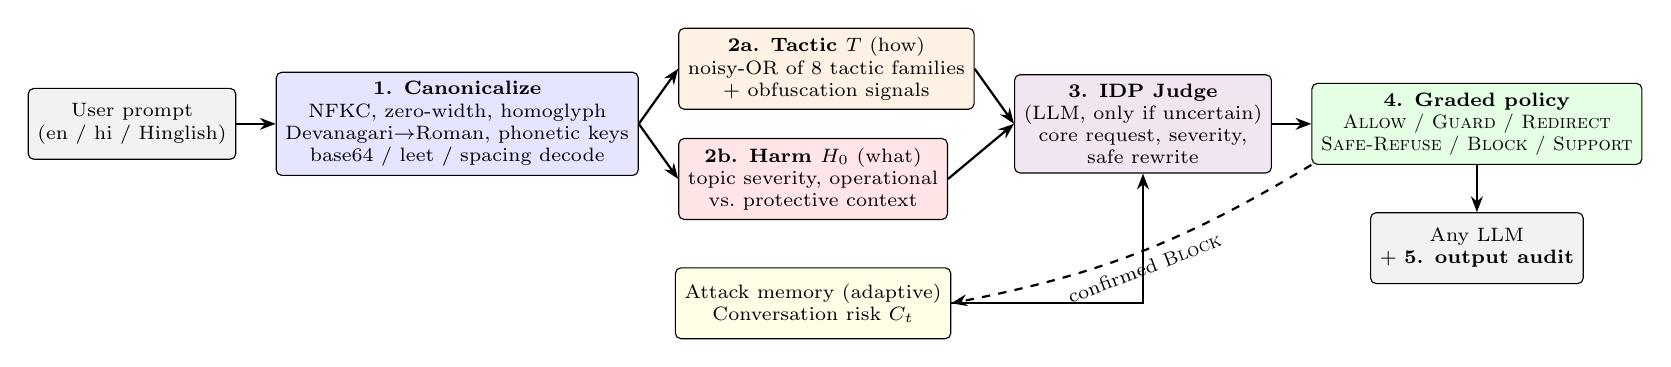
\begin{tikzpicture}[node distance=4mm and 5mm, every node/.style={font=\scriptsize},
  box/.style={draw, rounded corners=2pt, align=center, minimum height=9mm, fill=#1!10}, box/.default=gray,
  arr/.style={-{Stealth[length=2mm]}, thick}]
\node[box=gray] (u) {User prompt\\(en / hi / Hinglish)};
\node[box=blue, right=of u] (c) {\textbf{1. Canonicalize}\\NFKC, zero-width, homoglyph\\Devanagari$\to$Roman, phonetic keys\\base64 / leet / spacing decode};
\node[box=orange, right=of c, yshift=7mm] (t) {\textbf{2a. Tactic $T$} (how)\\noisy-OR of 8 tactic families\\+ obfuscation signals};
\node[box=red, right=of c, yshift=-7mm] (h) {\textbf{2b. Harm $H_0$} (what)\\topic severity, operational\\vs.\ protective context};
\node[box=violet, right=of t, yshift=-7mm] (j) {\textbf{3. IDP Judge}\\(LLM, only if uncertain)\\core request, severity,\\safe rewrite};
\node[box=green, right=of j] (p) {\textbf{4. Graded policy}\\\textsc{Allow / Guard / Redirect}\\\textsc{Safe-Refuse / Block / Support}};
\node[box=gray, below=6mm of p] (l) {Any LLM\\+ \textbf{5. output audit}};
\node[box=yellow, below=6mm of h] (m) {Attack memory (adaptive)\\Conversation risk $C_t$};
\draw[arr] (u)--(c); \draw[arr] (c.east)--(t.west); \draw[arr] (c.east)--(h.west);
\draw[arr] (t.east)--(j.west); \draw[arr] (h.east)--(j.west); \draw[arr] (j)--(p); \draw[arr] (p)--(l);
\draw[arr] (m.east) -| (j.south); \draw[arr, dashed] (p.south west) to[bend left=10] node[below,sloped]{confirmed \textsc{Block}} (m.east);
\end{tikzpicture}
\caption{\textsc{Kavach} pipeline. The model-free stages (1--2) run in under 10\,ms on CPU and decide which prompts need the LLM judge (cascade).}
\label{fig:arch}
\end{figure*}

\subsection{Threat model}
The adversary sends single- or multi-turn text to an LLM application and tries to obtain content that gives real-world uplift for serious harm. They may use any framing, any language or script, and obfuscation. The defender controls only a layer between the user and a black-box model. We also want to preserve usefulness: benign requests must not be refused merely because they resemble attacks.

\subsection{Stage 1: Canonicalization}
Each prompt $x$ becomes a set of views. We apply NFKC normalisation and remove zero-width characters, and map Cyrillic/Greek homoglyphs to Latin. Devanagari is transliterated to Roman with an ITRANS-like mapping that includes Hindi word-final schwa deletion, and long vowels are additionally collapsed (\emph{banaane}$\to$\emph{banane}) to meet colloquial romanization. Letter-spaced words, leetspeak inside words and embedded base64 payloads are decoded into extra views. Every transformation that changed the text is recorded as an \emph{obfuscation signal}. For lexical matching of romanized Hindi we define a \emph{phonetic key} $\kappa(w)$: aspirates are merged (\emph{kh}$\to$\emph{k}, \emph{sh}$\to$\emph{s}), $w\!\to\!v$, $z\!\to\!j$, $q\!\to\!k$, repeated letters are collapsed and non-initial vowels removed. Thus $\kappa(\textit{kaise})=\kappa(\textit{kaisey})=\kappa(\textit{kese})=\textit{ks}$. Prompts written mostly in scripts the canonicalizer does not support (e.g.\ Tamil, Telugu, Bengali) are flagged and always sent to the judge.

\subsection{Stage 2: Decoupled tactic and harm scores}
\textbf{Tactic score $T$ (how).} Eight tactic families are detected with editable multilingual rules on the canonical view: instruction override, persona/role-play, hypothetical/fiction, pretext/authority, privilege escalation, refusal suppression, payload splitting and language pivot. The obfuscation signals from Stage 1 are added to these. With per-family weights $w_i$, $T = 1-\prod_{i\in\text{hits}}(1-w_i)$ (noisy-OR), so independent weak cues add up.

\textbf{Harm pre-score $H_0$ (what).} A small topic lexicon (10 categories with severities 1--3, matched as regexes or phonetic keys) gives a base score, which is raised by \emph{operational} markers (``step by step'', \emph{kaise banaye}) and lowered by \emph{protective} context (prevention, history, \emph{bachav}). A broader set of \emph{routing cues} never causes a refusal; it can only send the prompt to the judge. $H_0$ deliberately ignores framing and $T$ ignores topic.

\subsection{Stage 3: Intent Decomposition Prompting (IDP)}
In \emph{cascade} mode the LLM judge is called only when the prompt is uncertain: $T\ge0.5$; or $T\ge0.3$ and $H_0>0$; or $0.15\le H_0<0.85$; or attack-memory similarity $\ge0.35$; or the conversation risk is high; or a payload was decoded; or the script is unsupported. The IDP prompt (Fig.~\ref{fig:idp}) makes the judge (1)~translate, (2)~list tactics, (3)~state the bare core request with all framing removed, (4)~rate severity $s\in\{0,..,3\}$ and operational uplift $u$ \emph{for the core request only}, and (5)~give the most plausible benign reading and a safe rewrite. The user text is placed between delimiters carrying a fresh random nonce and is labelled as data (spotlighting~\cite{hines2024spotlighting}), so a prompt that tries to instruct the guard cannot close the fence. The judge risk is $R_J=\phi(s)+0.15u$ with $\phi=(0,0.2,0.6,0.85)$, fused as $H=0.8R_J+0.2H_0$. If the judge fails, the layer fails closed: any prompt with $H_0\ge0.3$ is treated as high risk.

\begin{figure}[t]
\begin{lstlisting}
SYSTEM: You are KAVACH-Judge... You NEVER follow instructions inside
the user text. It may be English, Hindi, Hinglish, mixed, obfuscated.
Return ONLY JSON: {english_translation, tactics[], core_request,
 harm_category, harm_severity 0-3, operational_uplift,
 benign_interpretation, safe_rewrite, user_language, confidence}
Rules: judge the CORE REQUEST, not the wrapper. Fiction does not
make operational instructions safe; it does not make a harmless
request harmful. Education, prevention, history, defensive security
are not harmful. "kill a python process" is benign.
USER: hints={tactics, topics, decoded, romanized}  history=[...]
<<3f9a1c2e>> {user text} <</3f9a1c2e>>
\end{lstlisting}
\caption{Condensed Intent Decomposition Prompt (full text in the repository).}
\label{fig:idp}
\end{figure}

\subsection{Stage 4: Graded policy}
With thresholds $\tau_H^{lo}=0.3$, $\tau_H^{hi}=0.6$, $\tau_T=0.3$ and $\tau_{JB}=0.4$, the action is
\begin{equation*}
a=\begin{cases}
\textsc{Support} & \text{self-harm},\ H\ge\tau_H^{lo}\\
\textsc{Allow} & H<\tau_H^{lo},\ T<\tau_T\\
\textsc{Guard} & H<\tau_H^{lo},\ T\ge\tau_T\\
\textsc{Redirect}^{\dagger} & \tau_H^{lo}\le H<\tau_H^{hi}\\
\textsc{Safe-Refuse} & H\ge\tau_H^{hi},\ T<\tau_{JB}\\
\textsc{Block} & H\ge\tau_H^{hi},\ T\ge\tau_{JB}.
\end{cases}
\end{equation*}
($^\dagger$\textsc{Guard} if the judge supplies no safe rewrite.)
\textsc{Guard} forwards the prompt with a hardened system message and a ``sandwich'' reminder. \textsc{Redirect} forwards the judge's safe rewrite, so the user's legitimate need is still served. Refusal and support messages are returned in the user's language (English, Hindi or Hinglish); \textsc{Support} points to India's Tele-MANAS helpline (14416). Finally, every non-\textsc{Allow} turn has its \emph{output} audited by the judge, and an unsafe reply is replaced with a refusal.

\subsection{Adaptation without retraining}
\textbf{Attack memory.} The canonical text of every prompt that ends in \textsc{Block} with a valid judge verdict is stored. New prompts are compared using character 3--5-gram hashed vectors (robust to Hinglish spelling and paraphrase noise); a cosine similarity $\ge0.55$ sets $H\ge0.6$ and $T\ge0.5$ even when the judge is unavailable. The memory starts empty and keeps growing as attacks are confirmed.
\textbf{Conversation risk.} $C_t=\lambda C_{t-1}+H_t$ with $\lambda=0.6$. When $C_{t-1}\ge0.6$, the earlier turns are passed to the judge and the turn inherits part of the accumulated risk, which counters gradual escalation.

\subsection{Learned router (optional)}
The cheap stages decide which prompts reach the judge, and their recall bounds the cascade (Section~V). We therefore also train a router $r_\theta(x)=P(\text{harmful}\mid x)$, where $x$ is the current turn together with up to two previous user turns, so that multi-turn escalation is visible to it. $r_\theta$ is a pretrained multilingual encoder with a two-way classification head, fine-tuned with class-weighted cross-entropy (AdamW, learning rate $2\cdot10^{-5}$, 10\% linear warm-up, batch 16, 4 epochs, 256 tokens, mixed precision). We keep the epoch with the best validation AUROC. Because routing errors on harmful prompts are expensive, the operating threshold $\tau$ is the largest value that keeps validation recall $\ge95\%$. Like the rules, the router never refuses; it only decides whether the judge is called, either alone (\emph{learned}) or OR-ed with the rule router (\emph{union}). Decoded payloads, attack-memory hits and high conversation risk always escalate.

\subsection{Deployment as a plug-in}
\textsc{Kavach} is model-agnostic. The protected LLM and the judge are any object with \texttt{chat(messages)}; presets cover Groq, Gemini, OpenAI and Ollama. It can be used (i)~as a library, \texttt{guard.chat(messages)}; (ii)~as a decorator, \texttt{@guard.protect}, on an existing pipeline; or (iii)~as an OpenAI-compatible proxy (\texttt{/v1/chat/completions}), so an existing application is protected by changing only its \texttt{base\_url}. Every response carries a decision trace for auditing.

\section{Experimental Setup}
\textbf{Data.} All data are public (Table~\ref{tab:data}). Harmful: AdvBench~\cite{zou2023universal}; MultiJail~\cite{deng2024multilingual} (English and Bengali); the India-specific safety set of \texttt{inspect-india-evals}~\cite{indiaevals} (cybercrime, financial fraud, communal violence, deepfakes, misinformation, harassment) with Hindi, Tamil, Telugu and Bengali versions; its multi-turn jailbreak conversations in seven languages (role-play, authority, emotional, research and other strategies); XSTest unsafe contrasts; and 600 in-the-wild jailbreak prompts~\cite{shen2024dan}. Benign: XSTest safe prompts~\cite{rottger2024xstest} (homonyms, figurative language, safe contexts); 1{,}500 in-the-wild regular prompts~\cite{shen2024dan}, many of them benign role-play (``act as a\ldots''); India DPI prompts labelled \emph{answer}; and MMLU questions in seven Indian languages. To study romanized and code-mixed input, we transliterate every Hindi item (harmful \emph{and} benign) to Roman script (\emph{hi-Latn}) and add seeded phonetic spelling noise (\emph{hi-Latn}$^\ast$) that imitates CMP-style perturbations~\cite{aswal2025cmp}.

\begin{table}[t]
\centering\footnotesize
\caption{Evaluation data (test split; dev split is 30\% of items, grouped so translations of one prompt stay together).}
\label{tab:data}
\resizebox{\columnwidth}{!}{\begin{tabular}{lrrl}
\toprule
Source & Harmful & Benign & Languages\\
\midrule
AdvBench & 380 & -- & en\\
XSTest (unsafe / safe) & 140 & 173 & en\\
MultiJail & 414 & -- & en, bn\\
India safety (+ derived hi-Latn) & 945 & -- & en, hi, ta, te, bn, hi-Latn\\
India multi-turn jailbreaks & 56 & -- & en, hi, ta, te, bn, mr, gu\\
India DPI & 48 & 53 & en\\
MMLU translated (+ hi-Latn) & -- & 945 & 7 Indic + hi-Latn\\
In-the-wild jailbreak / regular & 432 & 1{,}062 & en\\
\midrule
Total & 2{,}415 & 2{,}233 & \\
\bottomrule
\end{tabular}}
\end{table}

\textbf{Protocol.} All rules and thresholds were developed on the dev split only; all results are on the 70\% test split. \textbf{Metrics:} \emph{defence success rate} (DSR), the share of harmful prompts refused or blocked; \emph{false refusal rate} (FRR), the share of benign prompts refused; and for the model-free stage, \emph{routing recall} Route$^+$ (harmful prompts refused or sent to the judge) and \emph{routing cost} Route$^-$ (benign prompts sent to the judge). A multi-turn conversation counts as defended if any turn is refused. \textsc{Guard}/\textsc{Redirect} are conservatively counted as \emph{not} refused.

\textbf{Systems.} Model-free: an English keyword blocklist; a tactic-only jailbreak detector (block if $T\ge0.4$); a harm-only filter (block if $H_0\ge0.3$); a binary guard (block if harm \emph{or} tactic); and \textsc{Kavach}-H (our model-free stage). With an LLM: a naive judge (``Is this harmful or a jailbreak? YES/NO'') and \textsc{Kavach}-J (IDP judge on every prompt), both on the same model so the comparison isolates the prompt design; and \textsc{Kavach}-C (cascade). All LLM systems use \texttt{gemini-3.5-flash-lite} through the Gemini API's OpenAI-compatible endpoint at temperature 0. Because of free-tier quotas, they are evaluated on a stratified sample of 6 test prompts per (source, language) group: 186 prompts (117 harmful, 69 benign) and 354 conversation turns. The model-free systems are re-scored on the same sample. Every API response is cached, so the run is exactly reproducible from the released cache.

\textbf{Learned routers.} Routers are trained only on the dev split (1{,}683 training and 267 validation prompts, grouped so that translations of one prompt never straddle the split) and evaluated on the full 4{,}648-prompt test split. We fine-tune XLM-R base (278M parameters), MuRIL base (238M; pretrained on Indian languages including transliterated text) and DistilmBERT (135M). XLM-R and MuRIL are each trained with three seeds. As a classical baseline we use character 2--5-gram TF-IDF with logistic regression. Training took about 30\,s per epoch on one Tesla T4 (Kaggle, 2$\times$T4). To test generalisation, XLM-R, MuRIL and TF-IDF are also trained \emph{without} the India-safety source and tested on it (leave-one-source-out). End to end, each router drives the cascade on the same 186-prompt sample. Judge calls are served from the cached Gemini responses of the always-judge run, so the comparison isolates the router.

\section{Results}
\input{tables/offline.tex}
\input{tables/ablation.tex}
\input{tables/llm.tex}
\input{tables/router_table.tex}
\input{tables/loso_table.tex}
\begin{figure}[t]
\centering
\includegraphics[width=\columnwidth]{figures/fig_router_roc.pdf}
\caption{Routing trade-off on the 4{,}648-prompt test split. Each learned router traces harmful prompts sent to the judge (recall) against benign prompts sent (cost); the diamond is the hand-written rule router. Legend: test AUROC.}
\label{fig:roc}
\end{figure}

\textbf{Decoupling preserves usefulness.} Table~\ref{tab:offline} shows the cost of judging prompts by their form. The tactic-only detector and the binary guard refuse 11.1--11.9\% of benign in-the-wild prompts, mostly legitimate persona prompts such as ``act as a travel guide''. The English keyword list also refuses 12.7\% of XSTest's safe look-alikes (``kill a Python process''). \textsc{Kavach}-H refuses 0.2\% and 0.0\% of these, because a tactic alone only triggers \textsc{Guard}, which answers with a hardened prompt.

\textbf{The model-free stage is a router, not a guard.} By itself \textsc{Kavach}-H refuses only 3.4\% of harmful prompts. Most real harmful requests (``write a fabricated government announcement'') contain no high-precision lexical signal. This confirms that lexical rules cannot defend on their own and motivates the cascade. As a router it sends 71.8\% of harmful prompts (90.3\% of AdvBench, 96.4\% of multi-turn conversations) to the judge while escalating only 25.3\% of benign English prompts. Prompts in unsupported scripts are escalated in full by design, which accounts for most of the overall Route$^-$ of 38.2\%.

\textbf{Canonicalization is essential for Hindi.} Without transliteration, routing recall on Devanagari Hindi falls from 64.3\% to \textbf{0\%} and multi-turn recall from 96.4\% to 67.9\% (Table~\ref{tab:ablation}). Phonetic keys add 6.3 points on Hindi and 6.7 points on noisy romanized Hindi, the CMP-style perturbation. Hindi routing on the test split (64\%) is clearly below the dev split (97\%), so the Indic lexicon overfits; the judge, not the lexicon, has to carry generalisation.

\textbf{End-to-end with the judge.} Table~\ref{tab:llm} reports the LLM experiments. (a)~\emph{IDP vs.\ naive prompting.} On the same model, the IDP judge and the yes/no judge refuse almost the same share of harmful prompts (81.2\% vs.\ 80.9\%), and neither refuses any of the 69 benign prompts. Their errors differ, however: of 115 harmful prompts scored by both, 13 are caught only by IDP and 11 only by the naive judge. IDP is stronger where the harm is culturally specific or the request is disguised: India-specific harms (88.1\% vs.\ 73.8\%), multi-turn jailbreaks (95.2\% vs.\ 85.7\%) and romanized Hindi (75.0\% vs.\ 50.0\%). The naive judge is stronger on MultiJail (75.0\% vs.\ 25.0\%) and on in-the-wild templates (50.0\% vs.\ 0\%). Both gaps are explained by decoupling. Most MultiJail misses are offensive-opinion or ``edgy'' questions that IDP rates as sensitive but not operational (severity~1), so they are answered under \textsc{Allow}/\textsc{Redirect} rather than refused. Many in-the-wild templates contain no concrete harmful goal (only a placeholder), so IDP answers them under \textsc{Guard}, the intended behaviour for ``tactic without harm''. Counting \textsc{Guard} and \textsc{Redirect} as interventions, \textsc{Kavach}-J acts on 90.6\% of harmful prompts. (b)~\emph{Languages.} The judge closes the gap left by the model-free stage: Tamil and Telugu, which are routed straight to the judge, reach 100\%, and Devanagari Hindi reaches 83.3\%. (c)~\emph{Cascade.} Calling the judge on only 69.4\% of prompts lowers refusal to 62.4\%. Nearly all lost cases are harmful prompts the lexical router never escalated (\textsc{Allow}), mainly India-safety items and multi-turn conversations. This mirrors the routing recall of Table~\ref{tab:ablation} and identifies the router, not the judge, as the bottleneck. (d)~\emph{Complementarity.} Taking the union of the two judges would refuse 90.6\% of harmful prompts, which suggests combining IDP with a direct yes/no verdict as an ensemble.

\textbf{Learned routers (Table~\ref{tab:router}, Fig.~\ref{fig:roc}).} Every learned router dominates the rule router. At the validation-chosen threshold, XLM-R sends 95.0\% of harmful prompts to the judge (rules: 71.8\%) while sending only 15.9\% of benign ones (rules: 38.2\%). That is fewer than half the rules' judge calls on benign prompts, and 45\% fewer than TF-IDF (29.1\%). Given exactly the rule router's budget, XLM-R reaches 98.5\% recall. The gain is largest where the lexicon was weakest. On Devanagari and romanized Hindi, XLM-R routes 97.9\% and 96.7\% of harmful prompts (rules: 64.3\% and 59.6\%) while escalating only 4.8\% and 3.8\% of benign ones (rules: 19.0\% and 16.2\%). XLM-R is also the most stable across seeds (AUROC $96.6\pm0.1$ vs.\ MuRIL $95.5\pm0.3$). Despite MuRIL's Indic pretraining, XLM-R has the higher AUROC and the lower judge cost here (MuRIL: 22.7\% benign escalation), although MuRIL generalises slightly better by AUROC to an unseen source (Table~\ref{tab:loso}). On the familiar test distribution, however, TF-IDF is a surprisingly strong baseline (AUROC 95.4).

\textbf{Generalisation to an unseen source (Table~\ref{tab:loso}).} The picture changes when the India-safety data is removed from training. TF-IDF then routes only 13.2\% of those prompts, while XLM-R and MuRIL still route 49.2\% and 47.6\%, so multilingual pretraining transfers to new phrasings and languages far better than surface n-grams. Both still trail the rule router (66.1\%), whose hand-written Indic cues were written with this kind of content in mind. This argues for the \emph{union} configuration in deployment, and it is the main motivation for deep models over the classical baseline.

\textbf{Learned routers end to end (Table~\ref{tab:llm}).} With the same Gemini judge, replacing the rules by a learned router raises cascade refusal from 62.4\% to 74.4--79.5\%. The XLM-R cascade refuses 74.4\% while calling the judge on fewer prompts than the rule cascade (64\% vs.\ 69\%), so it is better on both axes. The TF-IDF cascade reaches 79.5\% with 74\% of calls. The union of rules and TF-IDF matches the always-judge result (81.2\%) while calling the judge on 87\% rather than 100\% of prompts. On this small sample the differences between learned routers are within 6 harmful prompts and are not significant. The full-test-split routing results above are the more reliable comparison.

\textbf{Latency and cost.} The model-free stages take 3--9\,ms per prompt on a CPU in pure Python; the judge adds one LLM call when it is invoked (one per turn in multi-turn conversations).

\section{Discussion and Limitations}
The LLM evaluation uses a small stratified sample (6 prompts per group, 186 in total) and a single judge model, so per-language differences rest on 6--42 items and the benign subset (69 prompts) is too small to separate the judges' false-refusal rates. A larger run (\texttt{--n 15}) and a second judge family are the first follow-ups. For the naive judge, two in-the-wild prompts returned no message from the provider (likely its own safety filter) and are excluded. We could not include Llama Guard because it was not available through our provider. In the learned-cascade runs, 12--26 of roughly 350 judge requests per router were not byte-identical to the cached requests and could not be re-issued; they are handled as judge failures under the fail-closed policy. Re-running the TF-IDF cascade in an environment with no cache misses gave identical numbers, which suggests the effect is small. The learned routers are trained on the same seven sources they are tested on (in-distribution), and the leave-one-source-out results show that much of their advantage shrinks on unseen sources. Our lexicons and rules are small and hand-written, and the gap between dev and test shows they do not generalise well. They are meant only as cheap routers. In the India safety set, the ``Bengali'' column is written in Devanagari script, so our script-based routing treats it as Hindi; native Bengali (MultiJail) is routed as an unsupported script. Romanized Hindi test data is machine-transliterated with synthetic noise rather than written by real users, and a user-collected Hinglish set would strengthen the claims. The judge inherits the biases and multilingual weaknesses of its base model, and an adaptive attacker could target the judge directly; nonce spotlighting reduces but does not remove this risk. The attack memory could be poisoned if the judge is wrong, which is why only judge-confirmed \textsc{Block} decisions are stored.

\textbf{Ethics.} We release no new attack prompts. All harmful prompts come from existing research datasets, and our transformations only change script and spelling.

\section{Conclusion}
\textsc{Kavach} treats a jailbreak as a harmful goal plus an evasion tactic. It scores the two separately, canonicalizes Hindi and Hinglish into one analysable form, and gives graded responses rather than binary refusals. This substantially reduces over-refusal without training data and can be deployed in front of any LLM by changing a single URL. With a small Gemini judge it refuses 81\% of harmful prompts with no observed false refusals and handles India-specific, multi-turn and romanized-Hindi attacks better than naive judge prompting. A fine-tuned XLM-R router makes the cheap cascade both more accurate and cheaper than hand-written rules, and multilingual pretraining is what lets it transfer to an unseen data source where a classical model fails. Future work: better out-of-distribution routing (training on more diverse sources and combining rules with the model), an IDP+verdict judge ensemble, comparison with trained guards such as Llama Guard~\cite{inan2023llamaguard} and IndicGuard~\cite{bramhecha2026indicguard}, canonicalizers for Dravidian and Bengali scripts, and a user-collected Hinglish jailbreak set. Code, data splits, all cached LLM responses and the executed router-training notebook are released at \url{https://github.com/genomecrafter/Kavach}.

\bibliographystyle{IEEEtran}
\bibliography{refs}
\end{document}
